\section{Diskretne slucajne spremenljivke in porazdelitve}

\subsection{Diskretne slucajne spremenljivke}
X je realna funkcija s koncno ali \textbf{stevno} zalogo vrednosti $Z_X$\\
\underline{Porazdelitvena tabela}:\\
$Z_x=\{x_1, x_2, ...\}$\\
$X \sim
\begin{pmatrix}
    x_1 & x_2 & x_3 & \ldots \\
    p_1 & p_2 & p_3 & \ldots
\end{pmatrix} $\\\\
$P(X=x_i)=p_i$\\\\
$ 0\leq p_i \leq 1$ in $\Sigma p_i = 1$\\

\underline{Porazdelitvena funkcija}:\\
$F_X:\mathbb{R} \rightarrow [0, 1]$\\
$F_X(x)=P(X\leq x)$\\
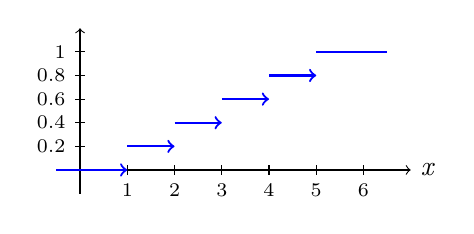
\begin{tikzpicture}[scale=0.6, graph1/.style={thick, color=blue}]	
    % Axis
    \draw[<-] (0,3)   -- (0,-0.5);
    \draw[->] (-0.5,0)-- (7,0) node[right] {$\mathit{x}$};	
    % x-axis
    \draw[-] (1, 0.1) -- (1,-0.1) node[below] {\scriptsize 1};
    \draw[-] (2, 0.1) -- (2,-0.1) node[below] {\scriptsize 2};
    \draw[-] (3, 0.1) -- (3,-0.1) node[below] {\scriptsize 3};
    \draw[-] (4, 0.1) -- (4,-0.1) node[below] {\scriptsize 4};
    \draw[-] (5, 0.1) -- (5,-0.1) node[below] {\scriptsize 5};
    \draw[-] (6, 0.1) -- (6,-0.1) node[below] {\scriptsize 6};
    % y-axis
    \draw[-] (-0.1,0.5) -- (0.1,0.5) (-0.1,0.5) node[left] {\scriptsize $0.2$};
    \draw[-] (-0.1,1) -- (0.1,1) (-0.1,1) node[left] {\scriptsize $0.4$};
    \draw[-] (-0.1,1.5) -- (0.1,1.5) (-0.1,1.5) node[left] {\scriptsize $0.6$};
    \draw[-] (-0.1,2) -- (0.1,2) (-0.1,2) node[left] {\scriptsize $0.8$};
    \draw[-] (0.1,2.5) -- (-0.1,2.5)  (-0.1,2.5)node[left] {\scriptsize $1$};
    Let us define some coordinates
        \draw[->,graph1] (-0.5,0) -- (1,0) node[right] {};
        \draw[->,graph1] (1,0.5) -- (2,0.5) node[right] {};
        \draw[->,graph1] (2,1) -- (3,1) node[right] {};
        \draw[->,graph1] (3,1.5) -- (4,1.5) node[right] {};
        \draw[->,graph1] (4,2) -- (5,2) node[right] {};
        \draw[-,graph1] (5,2.5) -- (6.5,2.5) node[right] {};
\end{tikzpicture} 

$\lim_{x\to\infty}F_X(x)=1$\\
$\lim_{x\to-\infty}F_X(x)=0$\\
$F_x \text{ je narascujoca}$\\
$\lim_{y\downarrow x}F_X(y)=F_X(x)$\\

\subsection{Bernoullijeva}
$X\sim B(p)$
\begin{itemize}[leftmargin=*]
\item V vsakem poskusu ima dogodek A verjetnost p, X ima vrednost 1, ce se je 
zgodil dogodek A, 0 sicer.
\item $P(X=1)=p, P(X=0)=1-p$
\item posebni primer Binomske za $n=1$
\end{itemize}

\subsection{Binomska}
$X\sim B(n,p)$
\begin{itemize}[leftmargin=*]
\item $X$ je \v stevilo pojavitev izida $A$ v $n$ ponovitvah poskusa.\\
$X_2$=st. lihih izidov pri 4 metih
\item $\displaystyle P(X=k)=\binom{n}{k}p^k (1-p)^{n-k}$\\ za $k=0,1,\ldots,n$.
\item R: $P(X=k)=\text{dbinom}(k,n,p), F_X(k)=\text{pbinom}(k,n,p)$.
\end{itemize}

\subsection{Geometrijska}
$X\sim G(p)$
\begin{itemize}[leftmargin=*]
\item $X$ je število ponovitev poskusa do (vključno) prve pojavitve izida $A$
$X_1$=st. poskusov da pade prvic 6
\item $\displaystyle P(X=k)=(1-p)^{k-1}p$\\ 
$\displaystyle P(X\le k) = 1 - (1-p)^k$\\$k=1,2,\ldots$
\item R: $P(X=k)=\text{dgeom}(k-1,p)\\ F_X(k)=\text{pgeom}(k-1,p)$.
\end{itemize}


\subsection{Pascalova/Negativna binomska}
$X\sim P(n,p)$
\begin{itemize}[leftmargin=*]
\item $X$ je število ponovitev poskusa do (vključno) $n$-te pojavitve izida $A$.\\
Npr. koliko poskusov rabimo do 10. sestice
\item $P(X=k)=\binom{k-1}{n-1}(1-p)^{k-n}p^n$\\$k=n,n+1,n+2,\ldots$
\item R: $P(X=k)=\text{dnbinom}(k-n,n,p)\\F_X(k)=\text{pnbinom}(k-n,n,p)$.
\end{itemize}


\subsection{Hipergeometrijska}
$X\sim H(R,B,n)$
\begin{itemize}[leftmargin=*]
    \item $X$ je število rdečih kroglic med izbranimi $n$ kroglicami
    \item $\displaystyle  P(X=k)=\frac{\binom{R}{k}\binom{B}{n-k}}{\binom{R+B}{n}}$\\$k=0,1,2,\ldots,\min\{n,R\}$.
    \item R: $P(X=k)=\text{dhyper}(k,R,B,n)\\F_X(k)=\text{phyper}(k,R,B,n)$.
\end{itemize}


\subsection{Poissonova}
$X\sim P(\lambda)$
\begin{itemize}[leftmargin=*]
\item V povprecju imamo na intervalu $\lambda$ ponovitev dogodka A
\item $X$ pa je število ponovitev dogodka $A$ na danem intervalu.
\item $\displaystyle  P(X=k)=\frac{\lambda^k}{k!}\cdot e^{-\lambda}$ za $k=0,1,2,\ldots$
\item R: $P(X=k)=\text{dpois}(k,\lambda)\\
F_X(k)=\text{ppois}(k,\lambda)$.
\end{itemize}

